% Import default values & document settings
% Layout settings
\newcommand{\FIITdefaultFontSize}[0] {12pt}
\setcounter{secnumdepth}{3}
\setcounter{tocdepth}{3}

% Language settings
% \newcommand{\FIITlanguage}[0] {slovak}
\newcommand{\FIITlanguage}[0] {slovak,english}
\def\FIITlagEN{}

% Global texts
\newcommand{\FIITuniversity}[0] {Slovak University of Technology in Bratislava}
\newcommand{\FIITuniversitySK}[0] {Slovenská technická univerzita v Bratislave}
\newcommand{\FIITfaculty}[0] {Faculty of informatics and information technologies}
\newcommand{\FIITfacultySK}[0] {Fakulta informatiky a informačných technológií}
\newcommand{\FIITthesis}[0] {Bachelor's thesis}
\newcommand{\FIITthesisSK}[0] {Bakalárska práca}
\newcommand{\FIITtitle}[0] {Practical usage of Zero-knowledge in different use-cases in blockchains}
\newcommand{\FIITtitleSK}[0] {Praktické využitie dôkazov s nulovým vedomím v rôznych prípadoch použitia v blockchainoch}
\newcommand{\FIITauthor}[0] {Lukáš Častven}
\newcommand{\FIITsupervisor}[0] {Ing. Kristián Košťál PhD.}
\newcommand{\FIITevidenceNumber}[0] {FIIT-16768-116160}
\newcommand{\FIITdate}[0] {May 2024}
\newcommand{\FIITdateSK}[0] {May 2024}
\newcommand{\FIITstudyProgram}[0] {Informatics}
\newcommand{\FIITstudyProgramSK}[0] {Informatika}
\newcommand{\FIITstudyField}[0] {Computer Science}
\newcommand{\FIITdegreeCourseSK}[0] {9.2.1 Informatika}
\newcommand{\FIITinstitute}[0] {Institute of Computer Engineering and Applied Informatics}
\newcommand{\FIITinstituteSK}[0] {Ústav počítačového inžinierstva a aplikovanej informatiky}
\newcommand{\FIITsignPlace}[0] {In Bratislava, }
\newcommand{\FIITsignPlaceSK}[0] {V Bratislave, }
\newcommand{\FIITsignDate}[0] {25.12.2023}
\newcommand{\FIITArchiveName}[0] {BP\_LukasCastven.zip}


% Setup document
\documentclass[\FIITdefaultFontSize,a4paper,twoside,openright,\FIITlanguage]{book}

% Load all necessary packages
\usepackage[final]{pdfpages}
\usepackage[utf8]{inputenc}
\usepackage[T1]{fontenc}
\usepackage[\FIITlanguage]{babel}
\usepackage[a4paper]{geometry}
\usepackage[
  left = \glqq,% 
  right = \grqq,% 
  leftsub = \glq,% 
  rightsub = \grq%
]{dirtytalk}
\usepackage[parfill]{parskip}
\usepackage{enumitem}
\usepackage{calc}
\usepackage{graphicx}
\usepackage{float}
\usepackage{csquotes}
\usepackage{longtable}
\usepackage{setspace}
\usepackage{tabularx}
\usepackage{fancyhdr}
\usepackage[backend=bibtex,sorting=none]{biblatex}
\usepackage{listing}
\usepackage{lscape}
\usepackage{afterpage}
\usepackage{hyperref}
\usepackage{bera}
\usepackage{listings}
\usepackage{xcolor}
\usepackage{lipsum}
\usepackage{minted}
\usepackage{tikz}
\usepackage{tocloft}

% Remove unnecessary gap between paragraph if large figure is inserted after them
\raggedbottom

% lscape.sty Produce landscape pages in a (mainly) portrait document.
\usepackage{lscape}

% Custom commands
\newcommand{\signaturespace}[2]{
  % #1 = width of the dotted line
  % #2 = legend
  \begingroup
  \renewcommand{\arraystretch}{0}
  \begin{tabular}[t]{cc}
    \hspace*{0pt}
    \cleaders\hbox{\kern.6pt.\kern.6pt}\hskip#1\relax
    \hspace*{0pt}
    \\[0.5cm]
    #2
  \end{tabular}
  \endgroup
}

\newcommand{\emptypage}{\newpage
  \thispagestyle{empty}
  \mbox{}
  \newpage}

% openright does not work :(
\let\tmp\oddsidemargin
\let\oddsidemargin\evensidemargin
\let\evensidemargin\tmp
\reversemarginpar


% Setup bibliography
\bibliography{bibliography}

% Page design
\pagestyle{fancy}
\lhead{\nouppercase{\leftmark}}
\chead{}
\rhead{}
\lfoot{}
\cfoot{\thepage}
\rfoot{}

\begin{document}

% Initialize document
% Layout
\setstretch{1.5}

% Bibliography
\ifx\FIITlagEN\undefined
  \defbibheading{references}[Zoznam použitej literatúry]{
    \chapter*{#1}
    \addcontentsline{toc}{chapter}{#1}
    \markboth{#1}{#1}
  }
  \defbibheading{referencessec}[Zoznam použitej literatúry]{
    \section*{#1}
    \markboth{#1}{#1}
  }
\else
  \defbibheading{references}[References]{
    \chapter*{#1}
    \addcontentsline{toc}{chapter}{#1}
    \markboth{#1}{#1}
  }
  \defbibheading{referencessec}[References]{
    \section*{#1}
    \markboth{#1}{#1}
  }
\fi

% Syntax highlighting
\setminted[]{linenos,tabsize=2,breaklines}
\colorlet{punct}{red!60!black}
\definecolor{background}{HTML}{EEEEEE}
\definecolor{delim}{RGB}{20,105,176}
\colorlet{numb}{magenta!60!black}

% Text highlighting
\makeatletter
\newenvironment{btHighlight}[1][]
{\begingroup\tikzset{bt@Highlight@par/.style={#1}}\begin{lrbox}{\@tempboxa}}
    {\end{lrbox}\bt@HL@box[bt@Highlight@par]{\@tempboxa}\endgroup}

\newcommand\btHL[1][]{%
  \begin{btHighlight}[#1]\bgroup\aftergroup\bt@HL@endenv%
    }
    \def\bt@HL@endenv{%
  \end{btHighlight}%   
  \egroup
}
\newcommand{\bt@HL@box}[2][]{%
  \tikz[#1]{%
    \pgfpathrectangle{\pgfpoint{1pt}{0pt}}{\pgfpoint{\wd #2}{\ht #2}}%
    \pgfusepath{use as bounding box}%
    \node[anchor=base west, fill=black!10,outer sep=0pt,inner xsep=1pt, inner ysep=-2pt, rounded corners=3pt, minimum height=\ht\strutbox+1pt,#1]{\raisebox{1pt}{\strut}\strut\usebox{#2}};
  }%
}
\makeatother

% TODO https://www.fiit.stuba.sk/buxus/docs/organizacia_studia/pokyny/ZP-clenenie-pokyny_2022.pdf
% Cover & title page
% Cover page
	\begin{center}
\thispagestyle{empty}
\ifx\FIITlagEN\undefined
{\Large \FIITuniversitySK}
\else
{\Large \FIITuniversity}
\fi
\par\end{center}{\Large \par}

\begin{center}
\ifx\FIITlagEN\undefined
{\Large \FIITfacultySK}
\else
{\Large \FIITfaculty}
\fi
\par\end{center}{\Large \par}

\smallskip{}

\begin{center}
\ifx\FIITlagEN\undefined
Evidenčné číslo: \FIITevidenceNumber
\else
Reg. No.: \FIITevidenceNumber
\fi
\par\end{center}
\vfill{}

\begin{center}
\textbf{\Large \FIITauthor}
\par\end{center}{\Large \par}

\medskip{}


\begin{center}
\ifx\FIITlagEN\undefined
\textbf{\LARGE \FIITtitleSK}
\else
\textbf{\LARGE \FIITtitle}
\fi
\par\end{center}{\huge \par}

\medskip{}


\begin{center}

\ifx\FIITlagEN\undefined
{\Large \FIITthesisSK}
\else
{\Large \FIITthesis}
\fi
\par\end{center}{\Large \par}

\vfill{}

\ifx\FIITlagEN\undefined
Vedúci záverečnej práce: \FIITsupervisor
\else
Thesis supervisor: \FIITsupervisor
\fi

\medskip{}

\ifx\FIITlagEN\undefined
\FIITdateSK
\else
\FIITdate
\fi

\pagenumbering{roman}
\emptypage





% Thesis title page
	\begin{center}
\thispagestyle{empty}
\ifx\FIITlagEN\undefined
{\Large \FIITuniversitySK}
\else
{\Large \FIITuniversity}
\fi
\par\end{center}{\Large \par}

\begin{center}
\ifx\FIITlagEN\undefined
{\Large \FIITfacultySK}
\else
{\Large \FIITfaculty}
\fi
\par\end{center}{\Large \par}

\smallskip{}

\begin{center}
\ifx\FIITlagEN\undefined
Evidenčné číslo: \FIITevidenceNumber
\else
Reg. No.: \FIITevidenceNumber
\fi
\par\end{center}
\vfill{}

\begin{center}
\textbf{\Large \FIITauthor}
\par\end{center}{\Large \par}

\medskip{}


\begin{center}
\ifx\FIITlagEN\undefined
\textbf{\LARGE \FIITtitleSK}
\else
\textbf{\LARGE \FIITtitle}
\fi
\par\end{center}{\huge \par}

\medskip{}


\begin{center}

\ifx\FIITlagEN\undefined
{\Large \FIITthesisSK}
\else
{\Large \FIITthesis}
\fi
\par\end{center}{\Large \par}

\vfill{}

\ifx\FIITlagEN\undefined
Študijný program: \FIITstudyProgramSK

Študijný odbor: \FIITdegreeCourseSK

Školiace pracovisko: \FIITinstituteSK

Vedúci záverečnej práce: \FIITsupervisor
\else
Study programme: \FIITstudyProgram

Study field: \FIITstudyField

Training workplace: \FIITinstitute

Thesis supervisor: \FIITsupervisor
\fi

\medskip{}

\ifx\FIITlagEN\undefined
\FIITdateSK
\else
\FIITdate
\fi

\emptypage


% Thesis assignment
\newpage
\thispagestyle{empty}
\begin{center}
    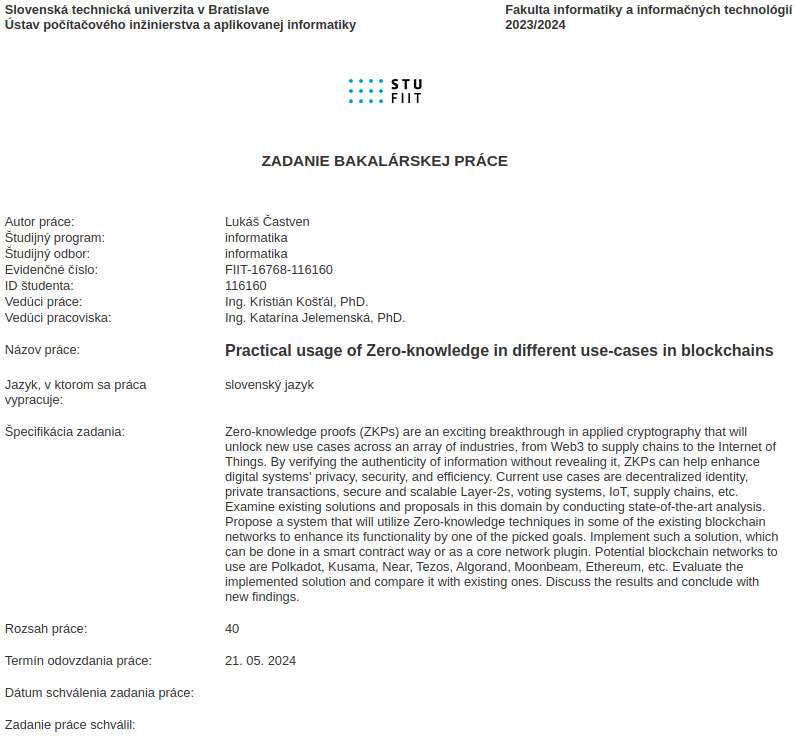
\includegraphics[scale=0.65]{assets/assignment.png}
\end{center}
\newpage
\emptypage

% Declaration of honor
% TODO
% \thispagestyle{empty}

\vspace*{\fill}

\ifx\FIITlagEN\undefined
\section*{Čestné prehlásenie}
\else
\section*{Declaration of honor}
\fi

\lipsum[3]

\ifx\FIITlagEN\undefined
\FIITsignPlaceSK \FIITsignDate
\else
\FIITsignPlace \FIITsignDate
\fi
\hspace*{\fill} \signaturespace{5cm}{\FIITauthor}

\emptypage

% Acknowledgements
% TODO
% \thispagestyle{empty}

\vspace*{\fill}

\ifx\FIITlagEN\undefined
\section*{Poďakovanie}
\else
\section*{Special thanks}
\fi

\lipsum[1]

\emptypage

% Annotation
% TODO add slovak
% Annotation in Slovak
\thispagestyle{empty}

\vspace*{\fill}

\section*{Anotácia}

\begin{minipage}[t]{1\columnwidth}
    \FIITuniversitySK

    \FIITfacultySK

    Študijný program: \FIITstudyProgramSK\\

    Autor: \FIITauthor

    \FIITthesisSK: \FIITtitleSK

    Vedúci projektu: \FIITsupervisor

    \FIITdateSK
\end{minipage}

\bigskip{}

Bakalárska práca skúma aplikáciu dôkazov s nulovým vedomím (ZKPs) v
blockchaine. Dôkazy s nulovým vedomím sú kryptografická metóda, ktorá
umožňuje overenie dát bez odhalenia samotných dát, čo je ideálne pre bezpečné
a súkromné aplikácie v blockchainoch. Táto práca je zameraná na návrh
a implementáciu konceptu schémy tajných adries s použitím ZKPs. Táto schéma
umožňuje odosielateľom odvodiť tajnú adresu z verejných údajov príjemcu.
Iba príjemca má kontrolu nad touto adresou, a zaroveň neodhaľuje žiadne informácie
o tom, kto príjemca je.

Výskum zahŕňa analýzu kryptografických princípov za ZKPs, nasledovanú
vysvetlením návrhu schémy tajných adries a jej integráciou do blockchainu Ethereum.

Táto práca prispieva do oblasti ukázaním, ako možno využiť ZKPs v blockchaine
na riešenie problémov súkromia, ponúkajúc riešenie vo forme konceptuálnej
implementácie schémy tajných adries s použitím ZKPs.

\newpage{}\thispagestyle{empty}\medskip{}

\emptypage

% Annotation in English
\thispagestyle{empty}

\vspace*{\fill}

\section*{Annotation}

\begin{minipage}[t]{1\columnwidth}
    \FIITuniversity

    \FIITfaculty

    Degree Course: \FIITstudyProgram\\

    Author: \FIITauthor

    \FIITthesis: \FIITtitle

    Supervisor: \FIITsupervisor

    \FIITdate
\end{minipage}

\bigskip{}

This bachelor's thesis investigates the application of Zero Knowledge Proofs
(ZKPs) in blockchains. Zero Knowledge Proofs are a cryptographic
method which enables the validation of data without revealing the
data itself, making it ideal for secure and private applications in
blockchain networks. The focus of this thesis is the design and implementation
of a proof of concept Stealth Address scheme using ZKPs. This scheme allows any sender to
derive a stealth address from recipients public data. Only the recipient has
control over this address, yet it does not leak any information about who the
recipient is.

The research includes an analysis of the cryptographic principles behind
ZKPs, followed by an explanation of the Stealth Address scheme's design and
its integration into a an Ethereum blockchain.

This thesis contributes to the field by showcasing how ZKPs can be utilized
in blockchain to address privacy concerns, offering a solution in the form of
a proof of concept  implementation of Stealth Address scheme using ZKPs.

\newpage{}\thispagestyle{empty}

\emptypage


% Table of contents
\ifx\FIITlagEN\undefined
    \renewcommand{\contentsname}{Obsah}
\else
    \renewcommand{\contentsname}{Table of contents}
\fi
\tableofcontents{}
\emptypage

% List of figures
\listoffigures
\emptypage

% List of tables
%\listoftables
%\emptypage

% List of abbreviations
\thispagestyle{plain}

\ifx\FIITlagEN\undefined
    \section*{\Huge Zoznam použitých skratiek}
    \markboth{Zoznam použitých skratiek}{Zoznam použitých skratiek}
\else
    \section*{\Huge List of abbreviations used}
    \markboth{List of abbreviations used}{List of abbreviations used}
\fi
\vskip 1cm

\begin{tabular}{ >{\bfseries}m{2cm} m{10cm} }
	AC  & Arithmetic Circuit       	\\
	ERC & Ethereum Request for Comments \\
	EVM & Ethereum Virtual Machine 	\\
	SNARK & Succinct Non-interactive Argument of Knowledge \\
	R1CS & Rank-1 Constraint System \\
	ZK  & Zero Knowledge           	\\
	ZKP & Zero Knowledge Proof
    % API		& Application Programming Interface \\
    % AWS		& Amazon Web Services \\
    % CNAME	& Canonical Name record \\
    % CSV		& Comma-Separated Values \\
    % DNS		& Domain Name System \\
    % HTTP	& Hyper-Text Transfer Protocol \\
    % ICANN	& Internet Corporation for Assigned Names and Numbers \\
    % IMAP	& Internet Message Access Protocol \\
    % IP		& Internet Protocol \\
    % JSON	& JavaScript Object Notation \\
    % MD5		& Message-Digest algorithm, version 5 \\
    % MSSQL	& Microsoft SQL \\
    % MX		& Mail Exchanger record \\
    % MySQL	& Maria SQL  \\
    % NS		& Name Server \\
    % OS		& Operating System \\
    % POP3    & Post Office Protocol, version 3\\
    % REST    & Representational state transfer \\
    % S3		& Amazon Simple Storage Service \\
    % SHA1	& Secure Hash Algorithm 1 \\
    % SMTP	& Simple Mail Transfer Protocol \\
    % SQL		& Structured Query Language \\
    % SRV		& Service record
\end{tabular}

\begin{tabular}{ >{\bfseries}m{2cm} m{10cm} }
    % TLD		& Top-Level Domain \\
    % TLS     & Transport Layer Security \\
    % URL		& Unified Resource Locator \\
    % XML		& Extensible Markup Language  
\end{tabular}

\emptypage


% Enable page numbering
\pagenumbering{arabic}

% Begin references segment
\begin{refsegment}
    \chapter{Introduction}

Zero Knowledge Proofs (ZKPs) are a powerful cryptography primitive. They allow
for the verification of a statement's truth without disclosing or in any way revealing
the actual content of the statement. This characteristic is crucial for
maintaining trust between parties while also preserving privacy.

The concept of ZKPs was first introduced in a 1989 research paper, "The
Knowledge Complexity of Interactive Proof Systems."\cite{Goldwasser1989}.
This work describes how in traditional proofs, such as demonstrating a graph
is Hamiltonian, more information is typically revealed than just the truth of
the theorem. This paper develops a computational complexity theory focusing
on the knowledge part within a proof. It introduces zero knowledge proofs,
a novel concept where proofs only confirm the correctness of a proposition
without exposing any extra knowledge. The paper focuses on interactive
proofs, where a dialogue between a prover and a verifier occurs. In these
interactive proofs, the prover aims to convince the verifier about the truth
of a private statement, with a very small probability of error. This
interaction is pivotal in ZKPs, as it allows for the verification of a
statement's truth without revealing the actual information or knowledge
behind the statement, maintaining the principle of conveying no
knowledge beyond the proposition's correctness.

This thesis extends the application of ZKPs to the concept of stealth
addresses in blockchain, as outlined in Vitalik Buterin's article "An
Incomplete Guide to Stealth Addresses."\cite{ButerinIncompleteGuide}.
Stealth addresses are critical for privacy on blockchains, allowing assets to
be transferred without revealing the recipient's identity and making
it difficult to link transactions to specific individuals.

Stealth addresses allow a sender (Alice) to transfer assets to a receiver (Bob) without
publicly revealing Bob's identity. To achieve this, Bob
must first provide a public meta stealth address generation data. This data
has different structure based on the underlying stealth address generation
schema. From this data Alice computes a new stealth address that only Bob can
control, and sends the assets to that newly generated address. Bob can then
access these assets from another address, only by providing a ZKP of given
address ownership.


    \emptypage

    \chapter{Analýza}
\par \lipsum[3]
\cite{coplienAOSDObjects}

\section{Podsekcia 1}

\begin{figure}[h!]
    \centering
    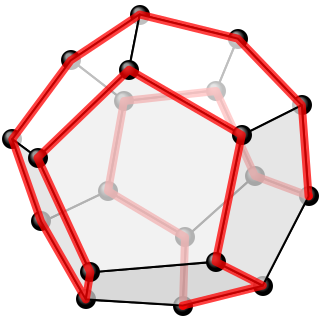
\includegraphics[width=\columnwidth]{assets/images/Hamiltonian_path_3d}
    \caption{Hamiltonovský graf}
    \label{fig:hamiltonian}
    \vspace{0.5cm}
\end{figure}

\par \lipsum[8]
\cite{opensourceArch}

\section{Podsekcia 2}
\par \lipsum[6]
\cite{coplienGOTODCI, coplienOredevDCI}
\par \lipsum[5]
\cite{generativeProg}
    \emptypage

    \chapter{Návrh riešenia}
\par \lipsum[3]

    \emptypage

    \chapter{Implementácia}
\par \lipsum[3]

    \emptypage

    \chapter{Testovanie}
\par \lipsum[3]

    \emptypage

    \chapter{Záver}
\par \lipsum[3]

\section{Zhodnotenie projektu}
\par \lipsum[3]

\section{Možné vylepšenia}
\par \lipsum[3]


    \ifx\FIITlagEN\undefined
    \else
        % Resume in Slovak
\thispagestyle{empty}

\begin{otherlanguage}{slovak}
\chapter*{Resumé}
\markboth{Resumé}{Resumé}
\addcontentsline{toc}{chapter}{Resumé} 

\end{otherlanguage}

    \fi

    % Bibliography
    \printbibliography[heading=references,segment=\therefsegment]

    % no page numbers for appendices
    \addtocontents{toc}{\protect\setcounter{tocdepth}{0}}
    \addtocontents{toc}{\cftpagenumbersoff{chapter}}

    \emptypage

\end{refsegment}

% Appendix
\appendix

\setcounter{figure}{0}
\setcounter{listing}{0}

\chapter{Polynomial zero test}
\label{appendix:zero_test}
\pagenumbering{arabic}
\renewcommand*{\thepage}{A-\arabic{page}}

\begin{refsegment}

The polynomial zero test is at the heart of the SNARK construction. Given a
polynomial $f \in \mathbb{F}_p^{\leq d}[X]$, the probability that a random
element $x \in \mathbb{F}_p$ is a root of $f$ is $d/p$.

\[ \Pr[f(x) = 0] \leq \frac{d}{p} \]

For example, $p = 2^{256}$ and $d = 2^{32}$, the probability that a random
element $x \in \mathbb{F}_p$ is a root of $f$ is $2^{224}$. This is a negligible
probability, and we can assume that $f$ is zero polynomial with high
probability when $f(x) = 0$ for a random $x \in \mathbb{F}_p$.

The generalization of the polynomial zero test for multivariate polynomials is
known as \textit{SZDL lemma}.

This can be used to prove that two polynomials are equal. Given two polynomials
$f, g$, we can evaluate $h = f - g$ at a random point $x$. If $h(x) = 0$, then
$f(x) - g(x) = 0 \Longrightarrow f(x) = g(x) \Longrightarrow f = g$ with high probability.

\printbibliography[heading=referencessec,segment=\therefsegment,resetnumbers=true]

\end{refsegment}


% Time schedule
\thispagestyle{empty}

\ifx\FIITlagEN\undefined
\chapter{Harmonogram práce}
\else
\chapter{Project task schedule}
\fi

\pagenumbering{arabic}
\renewcommand*{\thepage}{B-\arabic{page}}

\section{Zimný semester}

\begin{tabular}{|l||l|}
\hline
1\textsuperscript{st}-4\textsuperscript{th} week    & Consultations \& finding related research  \\
\hline
5\textsuperscript{th}-6\textsuperscript{th} week    & Working on the Introduction and Analysis chapters  \\
\hline
7\textsuperscript{th} week                          & Consultations  \\
\hline
8\textsuperscript{th}-10\textsuperscript{th} week   & Working on the Analysis chapters  \\
\hline
11\textsuperscript{th}-12\textsuperscript{th} week  & Working on the Solution proposal chapter \\
\hline
\end{tabular}

\section{Letný semester}

\begin{tabular}{|l||l|}
\hline
1\textsuperscript{st}-2\textsuperscript{nd} week    & Consultations \& designing API specification  \\
\hline
3\textsuperscript{rd}-6\textsuperscript{th} week    & Consultations \& implementation of back-end  \\
\hline
7\textsuperscript{th}-9\textsuperscript{th} week    & Implementation of server  \\
\hline
10\textsuperscript{th} week                         & Consultations \& implementation of front-end  \\
\hline
11\textsuperscript{th}-12\textsuperscript{th} week  & Finishing documentation \& solution testing  \\
\hline
\end{tabular}


% Contents of the digital medium
\thispagestyle{empty}

\ifx\FIITlagEN\undefined
    \chapter{Obsah digitálneho média}
\else
    \chapter{Contents of the digital medium}
\fi

\pagenumbering{arabic}
\renewcommand*{\thepage}{C-\arabic{page}}

\ifx\FIITlagEN\undefined
    \par Evidenčné číslo práce v informačnom systéme: \FIITevidenceNumber
\else
    \par Registration number of the thesis in the information system: \FIITevidenceNumber
\fi

\ifx\FIITlagEN\undefined
    \par Obsah digitálnej časti práce (archív ZIP):
\else
    \par Contents of the digital medium (ZIP archive):
\fi

% \begin{minted}[linenos=false]{text}
% Folder                  Contents
% /bin                    binárne súbory umožňujúce ...
%     /service
%     /app
% /models                 modely opísané v práci
%     modelA
%     modelB
% /scripts
% /data                   dátové množiny použité na ...
% /praca-pdf              pdf verzia záverečnej práce
%     /praca.pdf          pdf hlavná časť záverečnej práce
%     /prilohy.pdf        pdf textové prílohy záverečnej práce

% \end{minted}

% only if digital medium contents exceed 1 GB
% \par Digitálna časť práce má veľkosť 3.75 GB, kvôli čomu je uložená v systéme G Suite for Education.


\ifx\FIITlagEN\undefined
    \par Názov odovzdaného archívu: \FIITArchiveName.
\else
    \par Name of the submitted archive: \FIITArchiveName.
\fi


\end{document}
